\documentclass[12pt,openright,twoside,a4paper,brazil]{abntex2}
\SingleSpacing

\usepackage{graphicx}

\usepackage{ifxetex}
  \ifxetex
    \usepackage{fontspec}
    \defaultfontfeatures{Ligatures={TeX}}
  \else
    \usepackage[utf8]{inputenc}
    \usepackage[T1]{fontenc}
  \fi

\titulo{Modelo de relatório técnico escrito direto no latex}
\autor{Leonardo Goes Shibata}
\data{2020}
\instituicao{Banco Interamericano de Desenvolvimento}
\local{Sao Paulo}
\preambulo{BID-RT-2020-SAUDE-01, sigiloso}
\tipotrabalho{Relatório Técnico}


\begin{document}

%\imprimircapa
\imprimirfolhaderosto

\textual
\chapter{Introdução}
Esta é a introdução

\begin{figure}
  \caption{Pirâmide etária}
  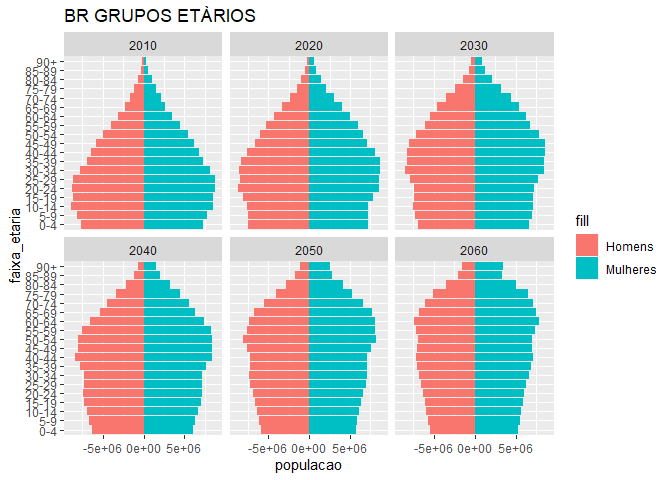
\includegraphics{plot-1.png}
  \legend{Fonte: elaboração própria}
\end{figure}


\end{document}

